\documentclass[12pt]{article}
\usepackage[]{graphicx}\usepackage[]{xcolor}
% maxwidth is the original width if it is less than linewidth
% otherwise use linewidth (to make sure the graphics do not exceed the margin)
\makeatletter
\def\maxwidth{ %
  \ifdim\Gin@nat@width>\linewidth
    \linewidth
  \else
    \Gin@nat@width
  \fi
}
\makeatother

\definecolor{fgcolor}{rgb}{0.345, 0.345, 0.345}
\newcommand{\hlnum}[1]{\textcolor[rgb]{0.686,0.059,0.569}{#1}}%
\newcommand{\hlstr}[1]{\textcolor[rgb]{0.192,0.494,0.8}{#1}}%
\newcommand{\hlcom}[1]{\textcolor[rgb]{0.678,0.584,0.686}{\textit{#1}}}%
\newcommand{\hlopt}[1]{\textcolor[rgb]{0,0,0}{#1}}%
\newcommand{\hlstd}[1]{\textcolor[rgb]{0.345,0.345,0.345}{#1}}%
\newcommand{\hlkwa}[1]{\textcolor[rgb]{0.161,0.373,0.58}{\textbf{#1}}}%
\newcommand{\hlkwb}[1]{\textcolor[rgb]{0.69,0.353,0.396}{#1}}%
\newcommand{\hlkwc}[1]{\textcolor[rgb]{0.333,0.667,0.333}{#1}}%
\newcommand{\hlkwd}[1]{\textcolor[rgb]{0.737,0.353,0.396}{\textbf{#1}}}%
\let\hlipl\hlkwb

\usepackage{framed}
\makeatletter
\newenvironment{kframe}{%
 \def\at@end@of@kframe{}%
 \ifinner\ifhmode%
  \def\at@end@of@kframe{\end{minipage}}%
  \begin{minipage}{\columnwidth}%
 \fi\fi%
 \def\FrameCommand##1{\hskip\@totalleftmargin \hskip-\fboxsep
 \colorbox{shadecolor}{##1}\hskip-\fboxsep
     % There is no \\@totalrightmargin, so:
     \hskip-\linewidth \hskip-\@totalleftmargin \hskip\columnwidth}%
 \MakeFramed {\advance\hsize-\width
   \@totalleftmargin\z@ \linewidth\hsize
   \@setminipage}}%
 {\par\unskip\endMakeFramed%
 \at@end@of@kframe}
\makeatother

\definecolor{shadecolor}{rgb}{.97, .97, .97}
\definecolor{messagecolor}{rgb}{0, 0, 0}
\definecolor{warningcolor}{rgb}{1, 0, 1}
\definecolor{errorcolor}{rgb}{1, 0, 0}
\newenvironment{knitrout}{}{} % an empty environment to be redefined in TeX

\usepackage{alltt}
\newcommand{\SweaveOpts}[1]{}  % do not interfere with LaTeX
\newcommand{\SweaveInput}[1]{} % because they are not real TeX commands
\newcommand{\Sexpr}[1]{}       % will only be parsed by R


\usepackage{amsmath}
\usepackage{graphicx,psfrag,epsf}
\usepackage{enumerate}
\usepackage{natbib}
%\usepackage{url} % not crucial - just used below for the URL 
\usepackage[colorlinks=true,linkcolor={blue},citecolor={blue},urlcolor={blue}]{hyperref}
\usepackage{longtable,ctable}
\usepackage{amssymb}
\usepackage{amsfonts}
\usepackage{multirow}
\usepackage{graphicx}
\usepackage{booktabs}
\usepackage{mathptmx}
\usepackage{setspace}
\usepackage[utf8]{inputenc}
\usepackage{pgf}
\usepackage{algorithm}
\usepackage{algpseudocode}
\usepackage{threeparttable}


%\pdfminorversion=4
% NOTE: To produce blinded version, replace "0" with "1" below.
\newcommand{\blind}{0}

% DON'T change margins - should be 1 inch all around.
\addtolength{\oddsidemargin}{-.5in}%
\addtolength{\evensidemargin}{-.5in}%
\addtolength{\textwidth}{1in}%
\addtolength{\textheight}{1.3in}%
\addtolength{\topmargin}{-.8in}%


\newcommand{\R}{R}
\newcommand{\gbsg}{gbsg}
%\def\FsNg{\hbox{FS}(M_{g})}
\def\FsNg{\hbox{FS-M}}
\def\hhat{\hat\theta(\hat{H})}
\def\hchat{\hat\theta(\hat{H}^{c})}
\def\hknow{\hat\theta(H)}
\def\hcknow{\hat\theta(H^{c})}

\def\hplim{\theta^{\dagger}(H)}
\def\hcplim{\theta^{\dagger}(H^{c})}

\def\hhplim{\theta^{\ddagger}(H)}
\def\hhcplim{\theta^{\ddagger}(H^{c})}

\def\hath{\widehat{H}}
\def\hathc{{\widehat{H}}^{c}}


\def\sumin{\sum_{i=1}^n}
\def\nsumin{n^{-1}\sum_{i=1}^n}

\newcommand{\indep}{\perp \!\!\! \perp}



\begin{document}





\begin{knitrout}
\definecolor{shadecolor}{rgb}{0.969, 0.969, 0.969}\color{fgcolor}\begin{kframe}
\begin{alltt}
\hlkwd{rm}\hlstd{(}\hlkwc{list} \hlstd{=} \hlkwd{ls}\hlstd{())}

\hlcom{# Local github}
\hlstd{codepath} \hlkwb{<-} \hlkwd{c}\hlstd{(}\hlstr{"/media/larryleon/My Projects/GitHub/Forest-Search/R/"}\hlstd{)}
\hlkwd{source}\hlstd{(}\hlkwd{paste0}\hlstd{(codepath,} \hlstr{"source_forestsearch_v0.R"}\hlstd{))}
\hlkwd{source_fs_functions}\hlstd{(}\hlkwc{file_loc} \hlstd{= codepath)}

\hlkwd{library}\hlstd{(kableExtra)}
\hlkwd{library}\hlstd{(knitr)}
\hlkwd{library}\hlstd{(ggplot2)}
\hlkwd{library}\hlstd{(gridExtra)}
\hlkwd{library}\hlstd{(cubature)}
\hlkwd{library}\hlstd{(aVirtualTwins)}
\hlkwd{library}\hlstd{(randomForest)}
\hlkwd{library}\hlstd{(survival)}
\hlkwd{library}\hlstd{(survminer)}
\hlkwd{library}\hlstd{(grf)}
\hlkwd{library}\hlstd{(policytree)}
\hlkwd{library}\hlstd{(data.table)}
\hlkwd{library}\hlstd{(plyr)}
\hlkwd{library}\hlstd{(dplyr)}
\hlkwd{library}\hlstd{(glmnet)}

\hlkwd{library}\hlstd{(cli)}

\hlkwd{library}\hlstd{(corrplot)}

\hlkwd{library}\hlstd{(table1)}
\end{alltt}
\end{kframe}
\end{knitrout}




\begin{knitrout}
\definecolor{shadecolor}{rgb}{0.969, 0.969, 0.969}\color{fgcolor}\begin{kframe}
\begin{alltt}
\hlstd{maxFollow} \hlkwb{<-} \hlnum{84}
\hlstd{cens.type} \hlkwb{<-} \hlstr{"weibull"}

\hlcom{# m1 -censoring adjustment}
\hlstd{muC.adj} \hlkwb{<-} \hlkwd{log}\hlstd{(}\hlnum{1.5}\hlstd{)}
\hlstd{k.z3} \hlkwb{<-} \hlnum{1}
\hlstd{k.treat} \hlkwb{<-} \hlnum{0.9}

\hlstd{z1_frac} \hlkwb{<-} \hlnum{0.25}  \hlcom{# Default model index 'm1' (The 1st quartile of z1=er)}
\hlstd{pH_super} \hlkwb{<-} \hlnum{0.125}  \hlcom{# non-NULL re-defines z1_frac}

\hlkwa{if} \hlstd{(}\hlkwd{is.null}\hlstd{(pH_super)) \{}
    \hlcom{# pH_check<-with(gbsg,mean(pgr<=quantile(pgr,c(z3_frac),1,0) &}
    \hlcom{# er<=quantile(er,z1_frac)))}
    \hlstd{pH_check} \hlkwb{<-} \hlkwd{with}\hlstd{(gbsg,} \hlkwd{mean}\hlstd{(meno} \hlopt{==} \hlnum{0} \hlopt{&} \hlstd{er} \hlopt{<=} \hlkwd{quantile}\hlstd{(er, z1_frac)))}
    \hlkwd{cat}\hlstd{(}\hlstr{"Underlying pH_super"}\hlstd{,} \hlkwd{c}\hlstd{(pH_check),} \hlstr{"\textbackslash{}n"}\hlstd{)}
\hlstd{\}}
\hlcom{# pH_super specified If pH_super then override z1_frac and find z1_frac to}
\hlcom{# yield pH_super}

\hlkwa{if} \hlstd{(}\hlopt{!}\hlkwd{is.null}\hlstd{(pH_super)) \{}
    \hlcom{# Approximate Z1 quantile to yield pH proportion}
    \hlstd{z1_q} \hlkwb{<-} \hlkwd{uniroot}\hlstd{(propH.obj4,} \hlkwd{c}\hlstd{(}\hlnum{0}\hlstd{,} \hlnum{1}\hlstd{),} \hlkwc{tol} \hlstd{=} \hlnum{1e-04}\hlstd{,} \hlkwc{pH.target} \hlstd{= pH_super)}\hlopt{$}\hlstd{root}
    \hlcom{# pH_check<-with(gbsg,mean(pgr<=quantile(pgr,c(z3_frac),1,0) &}
    \hlcom{# er<=quantile(er,z1_q)))}
    \hlstd{pH_check} \hlkwb{<-} \hlkwd{with}\hlstd{(gbsg,} \hlkwd{mean}\hlstd{(meno} \hlopt{==} \hlnum{0} \hlopt{&} \hlstd{er} \hlopt{<=} \hlkwd{quantile}\hlstd{(er, z1_q)))}
    \hlkwd{cat}\hlstd{(}\hlstr{"pH"}\hlstd{,} \hlkwd{c}\hlstd{(pH_check),} \hlstr{"\textbackslash{}n"}\hlstd{)}
    \hlstd{rel_error} \hlkwb{<-} \hlstd{(pH_super} \hlopt{-} \hlstd{pH_check)}\hlopt{/}\hlstd{pH_super}
    \hlkwa{if} \hlstd{(}\hlkwd{abs}\hlstd{(rel_error)} \hlopt{>=} \hlnum{0.1}\hlstd{)}
        \hlkwd{stop}\hlstd{(}\hlstr{"pH_super approximation relative error exceeds 10%"}\hlstd{)}
    \hlstd{z1_frac} \hlkwb{<-} \hlstd{z1_q}
    \hlkwd{cat}\hlstd{(}\hlstr{"Underlying pH_super"}\hlstd{,} \hlkwd{c}\hlstd{(pH_check),} \hlstr{"\textbackslash{}n"}\hlstd{)}
\hlstd{\}}
\end{alltt}
\begin{verbatim}
## pH 0.122449 
## Underlying pH_super 0.122449
\end{verbatim}
\begin{alltt}
\hlcom{# Bootstrap on log(hr) scale converted to HR (est.loghr=TRUE & est.scale='hr')}
\hlstd{t.start.all} \hlkwb{<-} \hlkwd{proc.time}\hlstd{()[}\hlnum{3}\hlstd{]}
\end{alltt}
\end{kframe}
\end{knitrout}


\begin{knitrout}
\definecolor{shadecolor}{rgb}{0.969, 0.969, 0.969}\color{fgcolor}\begin{kframe}
\begin{alltt}
\hlcom{######################### Forest search criteria}

\hlstd{hr.threshold} \hlkwb{<-} \hlnum{1.25}  \hlcom{# Initital candidates }
\hlstd{hr.consistency} \hlkwb{<-} \hlnum{1}  \hlcom{# Candidates for many splits}
\hlstd{pconsistency.threshold} \hlkwb{<-} \hlnum{0.9}
\hlstd{stop.threshold} \hlkwb{<-} \hlnum{0.95}
\hlstd{maxk} \hlkwb{<-} \hlnum{2}
\hlstd{nmin.fs} \hlkwb{<-} \hlnum{60}
\hlstd{pstop_futile} \hlkwb{<-} \hlnum{0.5}
\hlcom{# Limit timing for forestsearch}
\hlstd{max.minutes} \hlkwb{<-} \hlnum{3}
\hlstd{m1.threshold} \hlkwb{<-} \hlnum{Inf}  \hlcom{# Turning this off (Default)}
\hlcom{# pconsistency.threshold<-0.70 # Minimum threshold (will choose max among}
\hlcom{# subgroups satisfying)}
\hlstd{fs.splits} \hlkwb{<-} \hlnum{400}  \hlcom{# How many times to split for consistency}
\hlcom{# vi is % factor is selected in cross-validation --> higher more important}
\hlcom{# Null, turns off grf screening}
\hlstd{d.min} \hlkwb{<-} \hlnum{10}  \hlcom{# Min number of events for both arms (d0.min=d1.min=d.min)}
\hlcom{# default=5 Virtual twins analysis Counter-factual difference (C-E) >=}
\hlcom{# vt.threshold Large values in favor of C (control)}
\hlstd{vt.threshold} \hlkwb{<-} \hlnum{0.225}  \hlcom{# For VT delta}
\hlstd{treat.threshold} \hlkwb{<-} \hlnum{0}

\hlstd{maxdepth} \hlkwb{<-} \hlnum{2}
\hlstd{n.min} \hlkwb{<-} \hlnum{60}
\hlstd{ntree} \hlkwb{<-} \hlnum{1000}
\hlcom{# GRF criteria}
\hlstd{dmin.grf} \hlkwb{<-} \hlnum{12}  \hlcom{# For GRF delta}
\hlcom{# Note: For CRT this represents dmin.grf/2 RMS for control (-dmin.grf/2 for}
\hlcom{# treatment)}
\hlstd{frac.tau} \hlkwb{<-} \hlnum{0.6}

\hlstd{outcome.name} \hlkwb{<-} \hlkwd{c}\hlstd{(}\hlstr{"y.sim"}\hlstd{)}
\hlstd{event.name} \hlkwb{<-} \hlkwd{c}\hlstd{(}\hlstr{"event.sim"}\hlstd{)}
\hlstd{id.name} \hlkwb{<-} \hlkwd{c}\hlstd{(}\hlstr{"id"}\hlstd{)}
\hlstd{treat.name} \hlkwb{<-} \hlkwd{c}\hlstd{(}\hlstr{"treat"}\hlstd{)}

\hlstd{cox.formula.sim} \hlkwb{<-} \hlkwd{as.formula}\hlstd{(}\hlkwd{paste}\hlstd{(}\hlstr{"Surv(y.sim,event.sim)~treat"}\hlstd{))}
\hlstd{cox.formula.adj.sim} \hlkwb{<-} \hlkwd{as.formula}\hlstd{(}\hlkwd{paste}\hlstd{(}\hlstr{"Surv(y.sim,event.sim)~treat+v1+v2+v3+v4+v5"}\hlstd{))}
\end{alltt}
\end{kframe}
\end{knitrout}



\begin{knitrout}
\definecolor{shadecolor}{rgb}{0.969, 0.969, 0.969}\color{fgcolor}\begin{kframe}
\begin{alltt}
\hlstd{mod.harm} \hlkwb{<-} \hlstr{"alt"}
\hlstd{hrH.target} \hlkwb{<-} \hlnum{2}
\hlcom{# out.loc = NULL turns off file creation}
\hlstd{N} \hlkwb{<-} \hlnum{1000}
\hlstd{this.dgm} \hlkwb{<-} \hlkwd{get.dgm4}\hlstd{(}\hlkwc{mod.harm} \hlstd{= mod.harm,} \hlkwc{N} \hlstd{= N,} \hlkwc{k.treat} \hlstd{= k.treat,} \hlkwc{hrH.target} \hlstd{= hrH.target,}
    \hlkwc{cens.type} \hlstd{= cens.type,} \hlkwc{out.loc} \hlstd{=} \hlkwa{NULL}\hlstd{,} \hlkwc{details} \hlstd{=} \hlnum{TRUE}\hlstd{,} \hlkwc{parms_torand} \hlstd{=} \hlnum{FALSE}\hlstd{)}
\end{alltt}
\end{kframe}
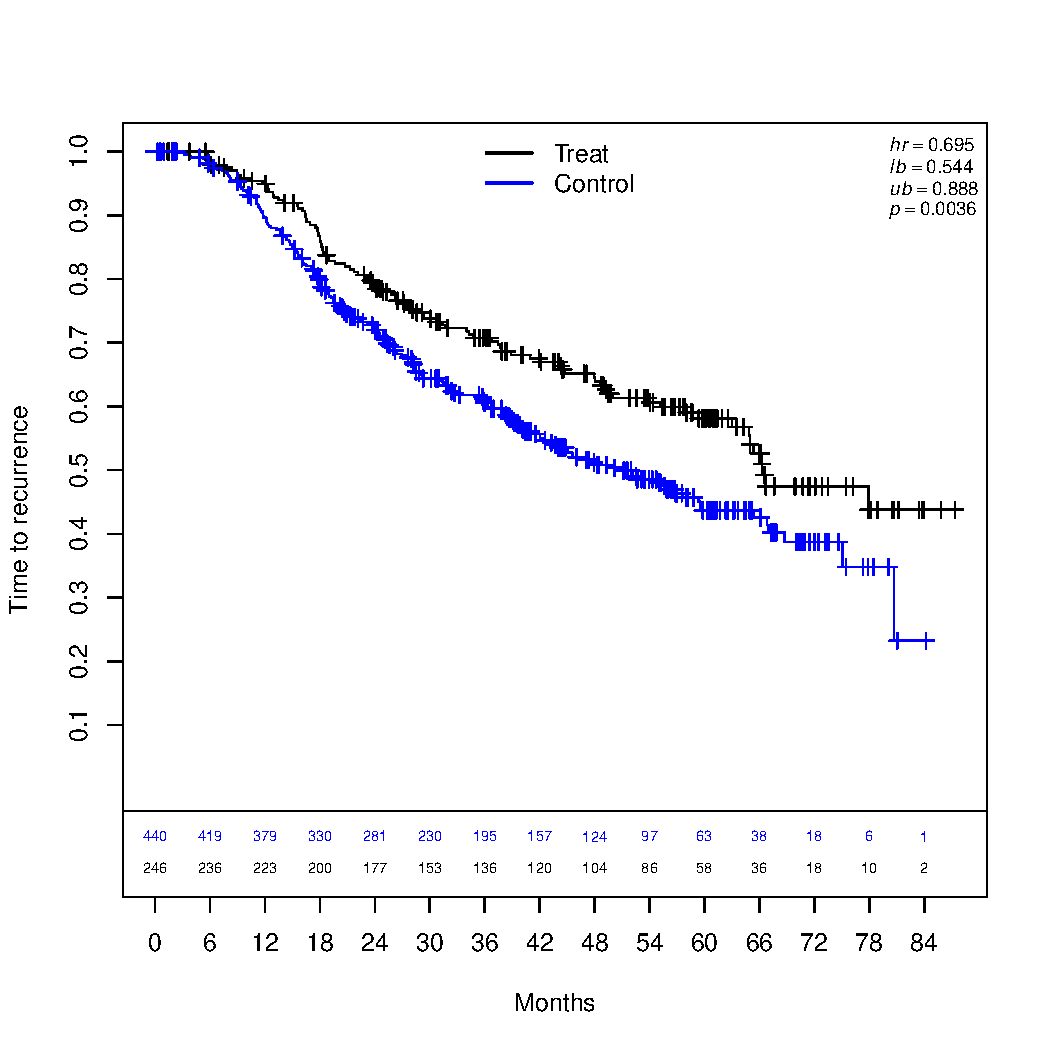
\includegraphics[width=\maxwidth]{figure/r_DGMsetup-1} 
\begin{kframe}\begin{verbatim}
## Super-population empirical harm and non-harm hazard ratios= 2.000007 0.6466405 
## Causal HR (empirical ITT)= 0.7057463
\end{verbatim}
\begin{alltt}
\hlstd{file_out} \hlkwb{<-} \hlkwd{c}\hlstd{(}\hlstr{"output/sim-FS4_N1k_Noise=3_hrH=2_sim99.Rdata"}\hlstd{)}
\end{alltt}
\end{kframe}
\end{knitrout}

\begin{knitrout}
\definecolor{shadecolor}{rgb}{0.969, 0.969, 0.969}\color{fgcolor}\begin{kframe}
\begin{alltt}
\hlcom{# sim sensH ppvH sensHc ppvHc lasso_omit 1: 78 0.4402985 0.5412844 0.9422633}
\hlcom{# 0.9158249 1 2: 164 0.6146789 0.5275591 0.9326599 0.9518900 1 3: 221 0.3149606}
\hlcom{# 0.5063291 0.9553265 0.9055375 1 4: 257 0.5528455 0.5666667 0.9407070}
\hlcom{# 0.9375000 1 5: 273 0.5422535 0.5065789 0.9125874 0.9233491 1}

\hlstd{n_add_noise} \hlkwb{<-} \hlnum{3}

\hlstd{sim} \hlkwb{<-} \hlnum{99}

\hlstd{dgm} \hlkwb{<-} \hlstd{this.dgm}\hlopt{$}\hlstd{dgm}

\hlstd{x} \hlkwb{<-} \hlkwd{sim_aftm4_gbsg}\hlstd{(}\hlkwc{dgm} \hlstd{= dgm,} \hlkwc{n} \hlstd{= N,} \hlkwc{maxFollow} \hlstd{= maxFollow,} \hlkwc{muC.adj} \hlstd{= muC.adj,} \hlkwc{simid} \hlstd{= sim)}

\hlstd{kmfit} \hlkwb{<-} \hlkwd{survfit}\hlstd{(}\hlkwd{Surv}\hlstd{(y.sim, event)} \hlopt{~} \hlstd{treat,} \hlkwc{data} \hlstd{= x)}

\hlkwd{ggsurvplot}\hlstd{(kmfit,} \hlkwc{data} \hlstd{= x,} \hlkwc{main} \hlstd{=} \hlstr{"K-M curves for simulated data"}\hlstd{,} \hlkwc{legend} \hlstd{=} \hlstr{"top"}\hlstd{,}
    \hlkwc{legend.title} \hlstd{=} \hlstr{"Treatment"}\hlstd{,} \hlkwc{legend.labs} \hlstd{=} \hlkwd{c}\hlstd{(}\hlstr{"Control"}\hlstd{,} \hlstr{"Experimental"}\hlstd{),} \hlkwc{palette} \hlstd{=} \hlstr{"grey"}\hlstd{,}
    \hlkwc{risk.table} \hlstd{=} \hlnum{TRUE}\hlstd{,} \hlkwc{risk.table.col} \hlstd{=} \hlstr{"strata"}\hlstd{)}
\end{alltt}
\end{kframe}
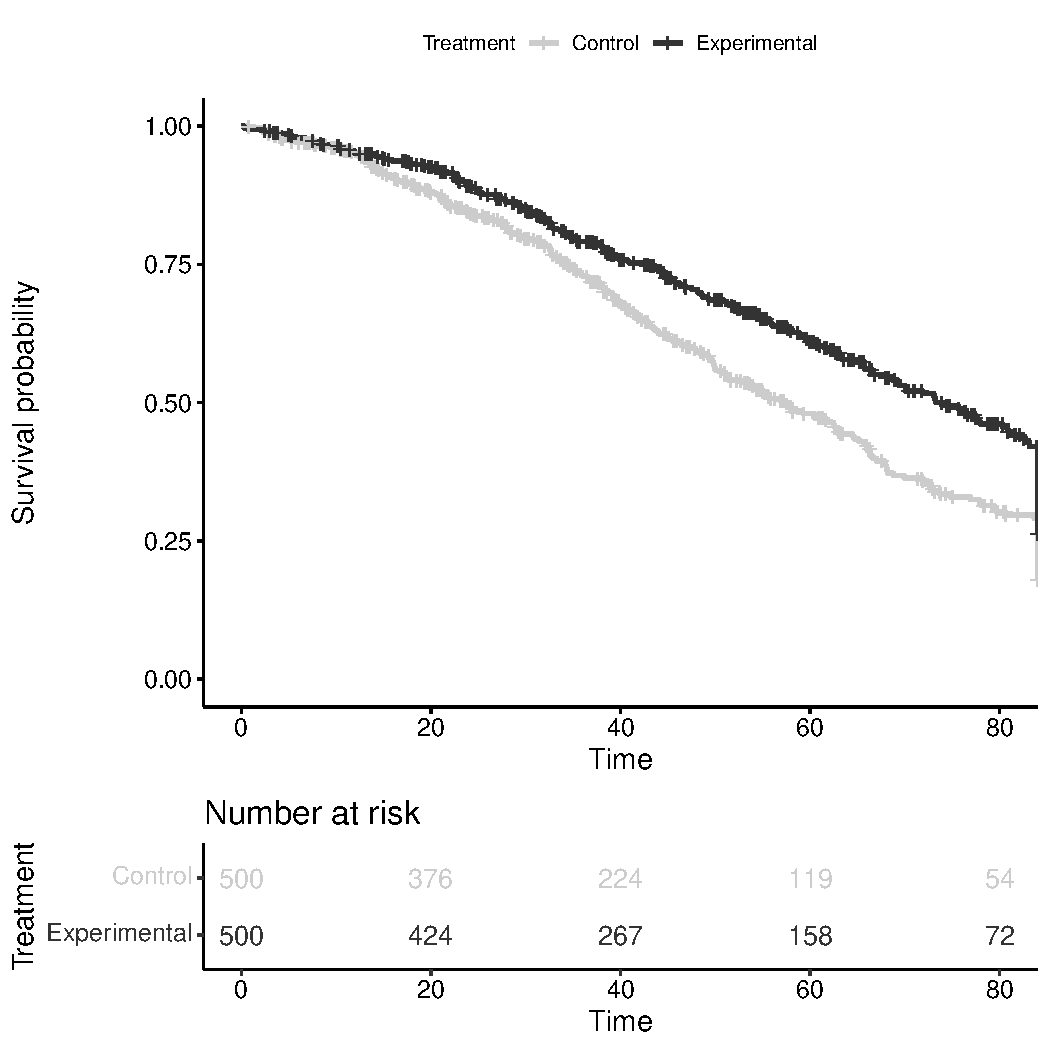
\includegraphics[width=\maxwidth]{figure/r_FSanalysis-1} 
\begin{kframe}\begin{alltt}
\hlkwa{if} \hlstd{(n_add_noise} \hlopt{==} \hlnum{0}\hlstd{) \{}
    \hlstd{confounders.name} \hlkwb{<-} \hlkwd{c}\hlstd{(}\hlstr{"z1"}\hlstd{,} \hlstr{"z2"}\hlstd{,} \hlstr{"z3"}\hlstd{,} \hlstr{"z4"}\hlstd{,} \hlstr{"z5"}\hlstd{,} \hlstr{"size"}\hlstd{,} \hlstr{"grade3"}\hlstd{)}
\hlstd{\}}

\hlkwa{if} \hlstd{(n_add_noise} \hlopt{==} \hlnum{5}\hlstd{) \{}
    \hlkwd{set.seed}\hlstd{(}\hlnum{8316951} \hlopt{+} \hlnum{1000} \hlopt{*} \hlstd{sim)}
    \hlcom{# Add 5 noise}
    \hlstd{x}\hlopt{$}\hlstd{noise1} \hlkwb{<-} \hlkwd{rnorm}\hlstd{(N)}
    \hlstd{x}\hlopt{$}\hlstd{noise2} \hlkwb{<-} \hlkwd{rnorm}\hlstd{(N)}
    \hlstd{x}\hlopt{$}\hlstd{noise3} \hlkwb{<-} \hlkwd{rnorm}\hlstd{(N)}
    \hlstd{x}\hlopt{$}\hlstd{noise4} \hlkwb{<-} \hlkwd{rnorm}\hlstd{(N)}
    \hlstd{x}\hlopt{$}\hlstd{noise5} \hlkwb{<-} \hlkwd{rnorm}\hlstd{(N)}
    \hlstd{confounders.name} \hlkwb{<-} \hlkwd{c}\hlstd{(}\hlstr{"z1"}\hlstd{,} \hlstr{"z2"}\hlstd{,} \hlstr{"z3"}\hlstd{,} \hlstr{"z4"}\hlstd{,} \hlstr{"z5"}\hlstd{,} \hlstr{"size"}\hlstd{,} \hlstr{"grade3"}\hlstd{,} \hlstr{"noise1"}\hlstd{,}
        \hlstr{"noise2"}\hlstd{,} \hlstr{"noise3"}\hlstd{,} \hlstr{"noise4"}\hlstd{,} \hlstr{"noise5"}\hlstd{)}
\hlstd{\}}

\hlkwa{if} \hlstd{(n_add_noise} \hlopt{==} \hlnum{3}\hlstd{) \{}
    \hlkwd{set.seed}\hlstd{(}\hlnum{8316951} \hlopt{+} \hlnum{1000} \hlopt{*} \hlstd{sim)}
    \hlcom{# Add 3 noise}
    \hlstd{x}\hlopt{$}\hlstd{noise1} \hlkwb{<-} \hlkwd{rnorm}\hlstd{(N,} \hlkwc{sd} \hlstd{=} \hlnum{1}\hlstd{)}
    \hlstd{x}\hlopt{$}\hlstd{noise2} \hlkwb{<-} \hlkwd{rnorm}\hlstd{(N,} \hlkwc{sd} \hlstd{=} \hlnum{1}\hlstd{)}
    \hlstd{x}\hlopt{$}\hlstd{noise3} \hlkwb{<-} \hlkwd{rnorm}\hlstd{(N,} \hlkwc{sd} \hlstd{=} \hlnum{1}\hlstd{)}
    \hlstd{confounders.name} \hlkwb{<-} \hlkwd{c}\hlstd{(}\hlstr{"z1"}\hlstd{,} \hlstr{"z2"}\hlstd{,} \hlstr{"z3"}\hlstd{,} \hlstr{"z4"}\hlstd{,} \hlstr{"z5"}\hlstd{,} \hlstr{"size"}\hlstd{,} \hlstr{"grade3"}\hlstd{,} \hlstr{"noise1"}\hlstd{,}
        \hlstr{"noise2"}\hlstd{,} \hlstr{"noise3"}\hlstd{)}
\hlstd{\}}

\hlcom{# More challenging which_replace <- which(confounders.name=='z1')}
\hlcom{# confounders.name[which_replace] <- 'er'}

\hlstd{cox.formula.check} \hlkwb{<-} \hlkwd{as.formula}\hlstd{(}\hlkwd{paste}\hlstd{(}\hlstr{"Surv(y.sim,event.sim)~treat+z1+z2+z3+z4+z5+size+grade3+noise1+noise2+noise3"}\hlstd{))}
\hlkwd{coxph}\hlstd{(cox.formula.check,} \hlkwc{data} \hlstd{= x)}
\end{alltt}
\begin{verbatim}
## Call:
## coxph(formula = cox.formula.check, data = x)
## 
##              coef  exp(coef)   se(coef)      z        p
## treat  -0.3407766  0.7112178  0.0882373 -3.862 0.000112
## z1      0.1454910  1.1566074  0.1074947  1.353 0.175905
## z2     -0.2671307  0.7655730  0.1447062 -1.846 0.064889
## z3      0.2355882  1.2656531  0.1481887  1.590 0.111883
## z4      0.5788410  1.7839696  0.1008861  5.738  9.6e-09
## z5     -0.9130836  0.4012849  0.0920592 -9.918  < 2e-16
## size   -0.0008376  0.9991627  0.0030755 -0.272 0.785347
## grade3 -0.1138499  0.8923919  0.1076257 -1.058 0.290132
## noise1  0.0565835  1.0582150  0.0447809  1.264 0.206386
## noise2 -0.0469701  0.9541160  0.0442398 -1.062 0.288365
## noise3  0.0063237  1.0063437  0.0402755  0.157 0.875237
## 
## Likelihood ratio test=181.3  on 11 df, p=< 2.2e-16
## n= 1000, number of events= 546
\end{verbatim}
\begin{alltt}
\hlstd{Zm} \hlkwb{<-} \hlkwd{cor}\hlstd{(}\hlkwd{as.matrix}\hlstd{(x[,} \hlkwd{c}\hlstd{(confounders.name)]))}
\hlkwd{corrplot}\hlstd{(Zm)}
\end{alltt}
\end{kframe}
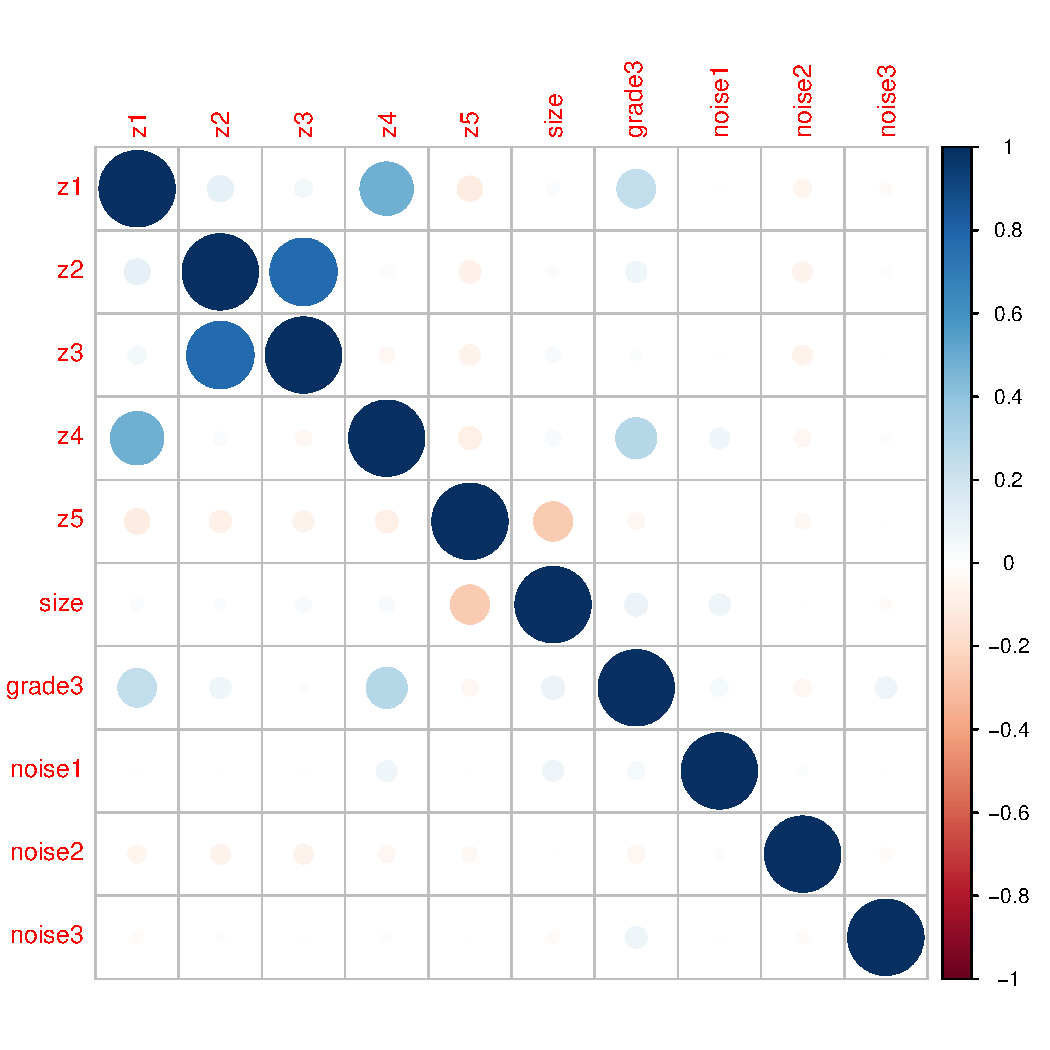
\includegraphics[width=\maxwidth]{figure/r_FSanalysis-2} 
\begin{kframe}\begin{alltt}
\hlkwd{suppressWarnings}\hlstd{(}\hlkwd{table1}\hlstd{(}\hlopt{~}\hlstd{z1} \hlopt{+} \hlstd{z2} \hlopt{+} \hlstd{z3} \hlopt{+} \hlstd{z4} \hlopt{+} \hlstd{z5} \hlopt{+} \hlstd{size} \hlopt{+} \hlstd{grade3} \hlopt{+} \hlstd{noise1} \hlopt{+} \hlstd{noise2} \hlopt{+}
    \hlstd{noise3} \hlopt{|} \hlstd{treat,} \hlkwc{data} \hlstd{= x))}
\end{alltt}
\end{kframe}
\begin{tabular}[t]{llll}
\toprule
  & 0 & 1 & Overall\\
\midrule
 & (N=500) & (N=500) & (N=1000)\\
\addlinespace[0.3em]
\multicolumn{4}{l}{\textbf{z1}}\\
\hspace{1em}Mean (SD) & 0.260 (0.439) & 0.250 (0.433) & 0.255 (0.436)\\
\hspace{1em}Median [Min, Max] & 0 [0, 1.00] & 0 [0, 1.00] & 0 [0, \vphantom{2} 1.00]\\
\addlinespace[0.3em]
\multicolumn{4}{l}{\textbf{z2}}\\
\hspace{1em}Mean (SD) & 0.518 (0.500) & 0.530 (0.500) & 0.524 (0.500)\\
\hspace{1em}Median [Min, Max] & 1.00 [0, 1.00] & 1.00 [0, 1.00] & 1.00 [0, \vphantom{1} 1.00]\\
\addlinespace[0.3em]
\multicolumn{4}{l}{\textbf{z3}}\\
\hspace{1em}Mean (SD) & 0.422 (0.494) & 0.402 (0.491) & 0.412 (0.492)\\
\hspace{1em}Median [Min, Max] & 0 [0, 1.00] & 0 [0, 1.00] & 0 [0, \vphantom{1} 1.00]\\
\addlinespace[0.3em]
\multicolumn{4}{l}{\textbf{z4}}\\
\hspace{1em}Mean (SD) & 0.512 (0.500) & 0.478 (0.500) & 0.495 (0.500)\\
\hspace{1em}Median [Min, Max] & 1.00 [0, 1.00] & 0 [0, 1.00] & 0 [0, 1.00]\\
\addlinespace[0.3em]
\multicolumn{4}{l}{\textbf{z5}}\\
\hspace{1em}Mean (SD) & 0.524 (0.500) & 0.528 (0.500) & 0.526 (0.500)\\
\hspace{1em}Median [Min, Max] & 1.00 [0, 1.00] & 1.00 [0, 1.00] & 1.00 [0, 1.00]\\
\addlinespace[0.3em]
\multicolumn{4}{l}{\textbf{size}}\\
\hspace{1em}Mean (SD) & 29.1 (14.7) & 27.6 (12.7) & 28.4 (13.7)\\
\hspace{1em}Median [Min, Max] & 25.0 [3.00, 120] & 25.0 [4.00, 100] & 25.0 [3.00, 120]\\
\addlinespace[0.3em]
\multicolumn{4}{l}{\textbf{grade3}}\\
\hspace{1em}Mean (SD) & 0.252 (0.435) & 0.200 (0.400) & 0.226 (0.418)\\
\hspace{1em}Median [Min, Max] & 0 [0, 1.00] & 0 [0, 1.00] & 0 [0, 1.00]\\
\addlinespace[0.3em]
\multicolumn{4}{l}{\textbf{noise1}}\\
\hspace{1em}Mean (SD) & 0.0194 (0.993) & -0.0855 (0.983) & -0.0331 (0.989)\\
\hspace{1em}Median [Min, Max] & 0.0198 [-3.14, 3.24] & -0.0674 [-3.65, 3.10] & -0.0172 [-3.65, 3.24]\\
\addlinespace[0.3em]
\multicolumn{4}{l}{\textbf{noise2}}\\
\hspace{1em}Mean (SD) & -0.00954 (0.953) & 0.0251 (0.976) & 0.00779 (0.964)\\
\hspace{1em}Median [Min, Max] & -0.0297 [-2.65, 2.95] & 0.0771 [-3.77, 2.73] & 0.0221 [-3.77, 2.95]\\
\addlinespace[0.3em]
\multicolumn{4}{l}{\textbf{noise3}}\\
\hspace{1em}Mean (SD) & 0.0238 (1.05) & -0.0404 (0.998) & -0.00830 (1.02)\\
\hspace{1em}Median [Min, Max] & 0.0381 [-3.07, 2.79] & -0.0336 [-3.00, 2.70] & 0.000560 [-3.07, 2.79]\\
\bottomrule
\end{tabular}

\begin{kframe}\begin{alltt}
\hlcom{# Options Allconfounders.name is list of confounders within analysis dataset}
\hlcom{# (1) use_lasso=TRUE & use_grf=FALSE Lasso used to possibly reduce dimension}
\hlcom{# Any continuous factors are cut at medians (2) use_lasso=TRUE & use_grf=TRUE}
\hlcom{# Lasso used to reduce dimension Continuous covariates are cut at medians}
\hlcom{# However, if GRF selects a covariate cut then only that cut is used: For}
\hlcom{# example if 'age <= median(ag)' is called for per Lasso but GRF includes 'age}
\hlcom{# <= 54', then only the latter is used (3) use_grf_only = TRUE (overrides}
\hlcom{# use_lasso and use_grf) Only factors selected via GRF are used (4) use_lasso =}
\hlcom{# F & use_grf =T Median cuts (unless selected via GRF) as in (2) However no}
\hlcom{# possible dimension reduction via lasso All categorical factors included (5)}
\hlcom{# If all options set to false, then all factors are included with continuous}
\hlcom{# factors cut at medians}

\hlstd{use_lasso} \hlkwb{<-} \hlnum{TRUE}
\hlstd{use_grf} \hlkwb{<-} \hlnum{TRUE}
\hlstd{use_grf_only} \hlkwb{<-} \hlnum{FALSE}

\hlstd{fs.est} \hlkwb{<-} \hlkwd{forestsearch}\hlstd{(}\hlkwc{df.analysis} \hlstd{= x,} \hlkwc{Allconfounders.name} \hlstd{= confounders.name,} \hlkwc{details} \hlstd{=} \hlnum{TRUE}\hlstd{,}
    \hlkwc{use_lasso} \hlstd{= use_lasso,} \hlkwc{use_grf} \hlstd{= use_grf,} \hlkwc{use_grf_only} \hlstd{= use_grf_only,} \hlkwc{dmin.grf} \hlstd{=} \hlnum{12}\hlstd{,}
    \hlkwc{frac.tau} \hlstd{=} \hlnum{0.6}\hlstd{,} \hlkwc{conf_force} \hlstd{=} \hlkwa{NULL}\hlstd{,} \hlkwc{outcome.name} \hlstd{= outcome.name,} \hlkwc{treat.name} \hlstd{= treat.name,}
    \hlkwc{event.name} \hlstd{= event.name,} \hlkwc{id.name} \hlstd{= id.name,} \hlkwc{n.min} \hlstd{= nmin.fs,} \hlkwc{hr.threshold} \hlstd{= hr.threshold,}
    \hlkwc{hr.consistency} \hlstd{= hr.consistency,} \hlkwc{fs.splits} \hlstd{= fs.splits,} \hlkwc{d0.min} \hlstd{= d.min,} \hlkwc{d1.min} \hlstd{= d.min,}
    \hlkwc{pstop_futile} \hlstd{= pstop_futile,} \hlkwc{pconsistency.threshold} \hlstd{= pconsistency.threshold,}
    \hlkwc{stop.threshold} \hlstd{= stop.threshold,} \hlkwc{max.minutes} \hlstd{= max.minutes,} \hlkwc{maxk} \hlstd{= maxk,} \hlkwc{by.risk} \hlstd{=} \hlnum{12}\hlstd{,}
    \hlkwc{plot.sg} \hlstd{=} \hlnum{TRUE}\hlstd{)}
\end{alltt}
\begin{verbatim}
## --------------------------------------------------------------------------------
## FS: GRF stage for cut selection with dmin,tau= 12 0.6 
## --------------------------------------------------------------------------------
## tau, maxdepth= 49.15213 2 
##   leaf.node control.mean control.size control.se treated.mean treated.size
## 1         2     2.611008   189.000000   1.807998    -2.611008   189.000000
## 2         3    -4.273379   811.000000   1.011238     4.273379   811.000000
## 3         4    -7.433748   488.000000   1.216630     7.433748   488.000000
## 4         5     2.558461   100.000000   2.934459    -2.558461   100.000000
## 5         6    -3.450438   296.000000   1.551139     3.450438   296.000000
## 6         7    12.249335   116.000000   2.849731   -12.249335   116.000000
##   treated.se       diff Nsg depth
## 1   1.807998   5.222015 189     1
## 2   1.011238  -8.546758 811     1
## 3   1.216630 -14.867497 488     2
## 4   2.934459   5.116922 100     2
## 5   1.551139  -6.900876 296     2
## 6   2.849731  24.498669 116     2
##   leaf.node control.mean control.size control.se treated.mean treated.size
## 6         7    12.249335   116.000000   2.849731   -12.249335   116.000000
##   treated.se     diff Nsg depth
## 6   2.849731 24.49867 116     2
## --------------------------------------------------------------------------------
## GRF subgroup found
## All splits
## [1] "z3 <= 0"        "noise3 <= 0.89" "z1 <= 0"       
## Terminating node at max.diff (sg.harm.id)
## [1] "z1 <= 0"
## --------------------------------------------------------------------------------
## # of continuous/categorical characteristics 4 6 
## Continuous characteristics: size noise1 noise2 noise3 
## Categorical characteristics: z1 z2 z3 z4 z5 grade3 
## CV lambda = 0.02782646 
## 10 x 1 sparse Matrix of class "dgCMatrix"
##                 s0
## z1      0.04420163
## z2      .         
## z3      .         
## z4      0.49151069
## z5     -0.77713914
## size    .         
## grade3  .         
## noise1  0.01624411
## noise2  .         
## noise3  .         
## Cox-LASSO selected: z1 z4 z5 noise1 
## Cox-LASSO not selected: z2 z3 size grade3 noise2 noise3 
## Median cuts after Lasso: noise1 
## Categorical after Lasso: z1 z4 z5 
## Factors per GRF: z3 <= 0 noise3 <= 0.89 z1 <= 0 
## Medians prior to removing if also in GRF: noise1 
## Factors after removing any duplicates also in GRF: noise1 
## ***Factors per lasso after omitting GRF dups***=z1
## ***Factors per lasso after omitting GRF dups***=z4
## ***Factors per lasso after omitting GRF dups***=z5
## ***Factors per lasso after omitting GRF dups***=noise1 <= median(noise1)
## Initial GRF cuts included z3 <= 0 noise3 <= 0.89 z1 <= 0 
## Factors included per GRF (not in lasso) z3 <= 0 noise3 <= 0.89 
## --------------------------------------------------------------------------------
## # of candidate subgroup factors= 6 
## [1] "noise1 <= median(noise1)" "noise3 <= 0.89"          
## [3] "z1"                       "z4"                      
## [5] "z5"                       "z3 <= 0"                 
## --------------------------------------------------------------------------------
## ***FSdata completed***=
## LMAX= 6 
## Confounders per grf screening q6 q1 q3 q5 q2 q4 
##   FSconfounders.name      vi.cs
## 6                 q6 0.39296139
## 1                 q1 0.16563376
## 3                 q3 0.13754508
## 5                 q5 0.13588252
## 2                 q2 0.08652653
## 4                 q4 0.08145071
## Number of unique levels (L) and possible subgroups= 12 4095 
## # of subgroups based on # variables > k.max and excluded (per million) 0.004017 
## k.max= 2 
## Events criteria for control,exp= 10 10 
## # of subgroups with events less than criteria: control, experimental 7 7 
## # of subgroups with sample size less than criteria 8 
## # of subgroups meeting all criteria = 70 
## # of subgroups fitted (Cox model estimable) = 70 
## *Subgroup Searching Minutes=* 0.00335 
## Number of subgroups meeting HR threshold 2 
## --------------------------------------------------------------------------------
## Subgroup candidate(s) found (FS)
## --------------------------------------------------------------------------------
## # of candidate subgroups (meeting HR criteria) =  2 
## Subgroups (1st 10) meeting overall screening thresholds (HR, m1) sorted by HRs= Inf 
##      K   n   E d1    m1    m0   HR L(HR) U(HR) q6.0 q6.1 q1.0 q1.1 q3.0 q3.1
##  1:  2 116  85 48 22.39 40.90 2.36  1.53  3.66    1    0    0    0    0    1
##  2:  2 194 135 65 29.65 40.52 1.30  0.93  1.83    1    0    0    0    0    0
##  3: NA  NA  NA NA    NA    NA   NA    NA    NA   NA   NA   NA   NA   NA   NA
##  4: NA  NA  NA NA    NA    NA   NA    NA    NA   NA   NA   NA   NA   NA   NA
##  5: NA  NA  NA NA    NA    NA   NA    NA    NA   NA   NA   NA   NA   NA   NA
##  6: NA  NA  NA NA    NA    NA   NA    NA    NA   NA   NA   NA   NA   NA   NA
##  7: NA  NA  NA NA    NA    NA   NA    NA    NA   NA   NA   NA   NA   NA   NA
##  8: NA  NA  NA NA    NA    NA   NA    NA    NA   NA   NA   NA   NA   NA   NA
##  9: NA  NA  NA NA    NA    NA   NA    NA    NA   NA   NA   NA   NA   NA   NA
## 10: NA  NA  NA NA    NA    NA   NA    NA    NA   NA   NA   NA   NA   NA   NA
##     q5.0 q5.1 q2.0 q2.1 q4.0 q4.1
##  1:    0    0    0    0    0    0
##  2:    0    0    0    0    0    1
##  3:   NA   NA   NA   NA   NA   NA
##  4:   NA   NA   NA   NA   NA   NA
##  5:   NA   NA   NA   NA   NA   NA
##  6:   NA   NA   NA   NA   NA   NA
##  7:   NA   NA   NA   NA   NA   NA
##  8:   NA   NA   NA   NA   NA   NA
##  9:   NA   NA   NA   NA   NA   NA
## 10:   NA   NA   NA   NA   NA   NA
## Consistency 1 
## # of splits= 400 
## Model, % Consistency Met= !{z3 <= 0} {z1} 1 
## Number of subgroups meeting consistency criteria= 
##    Pcons   N g m K        M.1  M.2
## 1:     1 116 1 1 2 !{z3 <= 0} {z1}
\end{verbatim}
\end{kframe}
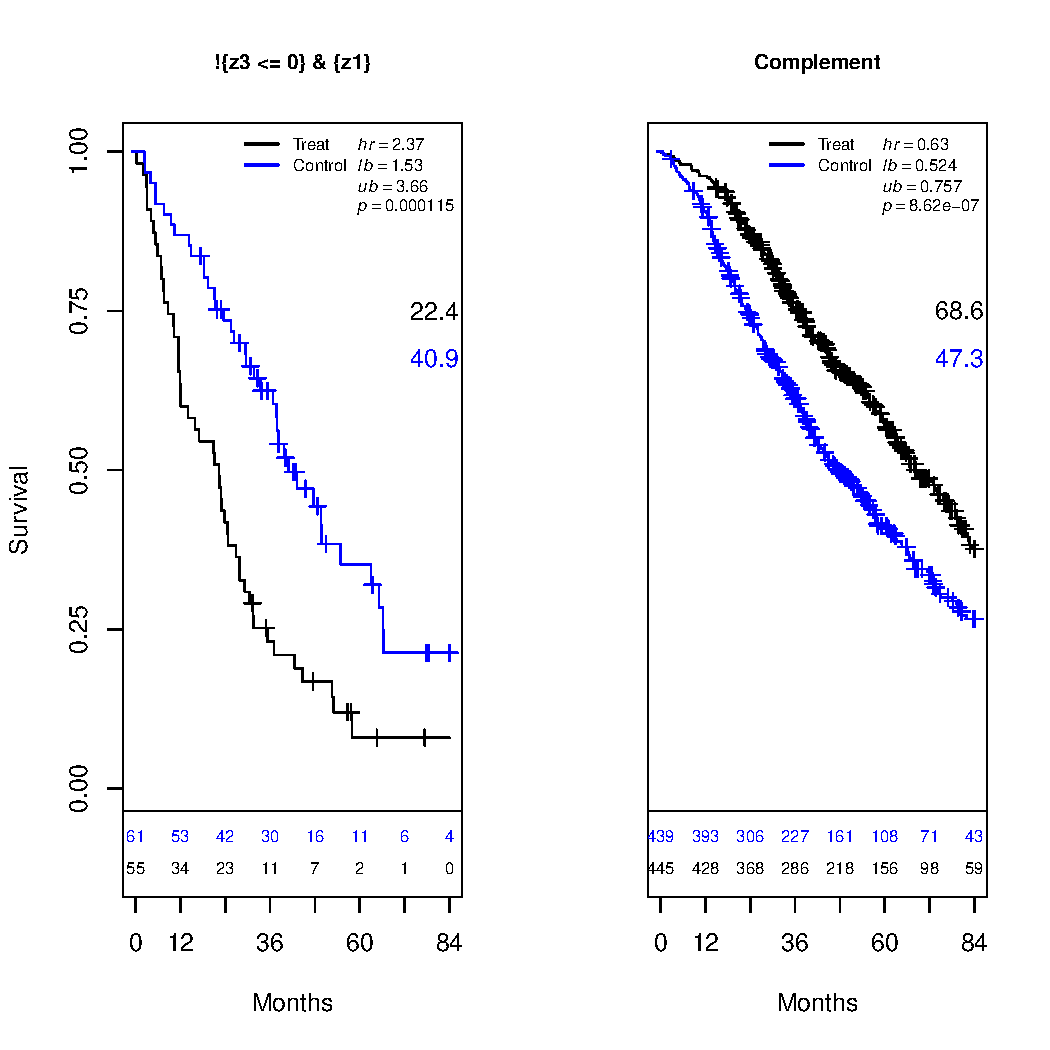
\includegraphics[width=\maxwidth]{figure/r_FSanalysis-3} 
\begin{kframe}\begin{verbatim}
## [1] "!{z3 <= 0}" "{z1}"      
## % consistency criteria met= 1 
## SG focus= hr 
## Subgroup Consistency Minutes= 0.02336667 
## --------------------------------------------------------------------------------
## Subgroup found (FS)
## --------------------------------------------------------------------------------
## Minutes overall= 0.05663333
\end{verbatim}
\begin{alltt}
\hlstd{grf.est} \hlkwb{<-} \hlkwd{grf.subg.harm.survival}\hlstd{(}\hlkwc{data} \hlstd{= x,} \hlkwc{confounders.name} \hlstd{= confounders.name,}
    \hlkwc{outcome.name} \hlstd{= outcome.name,} \hlkwc{event.name} \hlstd{= event.name,} \hlkwc{id.name} \hlstd{= id.name,} \hlkwc{treat.name} \hlstd{= treat.name,}
    \hlkwc{n.min} \hlstd{= n.min,} \hlkwc{dmin.grf} \hlstd{= dmin.grf,} \hlkwc{frac.tau} \hlstd{=} \hlnum{0.6}\hlstd{,} \hlkwc{details} \hlstd{=} \hlnum{TRUE}\hlstd{)}
\end{alltt}
\begin{verbatim}
## tau, maxdepth= 49.15213 2 
##   leaf.node control.mean control.size control.se treated.mean treated.size
## 1         2     2.611008   189.000000   1.807998    -2.611008   189.000000
## 2         3    -4.273379   811.000000   1.011238     4.273379   811.000000
## 3         4    -7.433748   488.000000   1.216630     7.433748   488.000000
## 4         5     2.558461   100.000000   2.934459    -2.558461   100.000000
## 5         6    -3.450438   296.000000   1.551139     3.450438   296.000000
## 6         7    12.249335   116.000000   2.849731   -12.249335   116.000000
##   treated.se       diff Nsg depth
## 1   1.807998   5.222015 189     1
## 2   1.011238  -8.546758 811     1
## 3   1.216630 -14.867497 488     2
## 4   2.934459   5.116922 100     2
## 5   1.551139  -6.900876 296     2
## 6   2.849731  24.498669 116     2
##   leaf.node control.mean control.size control.se treated.mean treated.size
## 6         7    12.249335   116.000000   2.849731   -12.249335   116.000000
##   treated.se     diff Nsg depth
## 6   2.849731 24.49867 116     2
## --------------------------------------------------------------------------------
## GRF subgroup found
## All splits
## [1] "z3 <= 0"        "noise3 <= 0.89" "z1 <= 0"       
## Terminating node at max.diff (sg.harm.id)
## [1] "z1 <= 0"
## --------------------------------------------------------------------------------
\end{verbatim}
\begin{alltt}
\hlcom{# plot(grf.est$tree)}
\end{alltt}
\end{kframe}
\end{knitrout}


\begin{knitrout}
\definecolor{shadecolor}{rgb}{0.969, 0.969, 0.969}\color{fgcolor}\begin{kframe}
\begin{alltt}
\hlkwd{library}\hlstd{(doParallel)}
\hlkwd{registerDoParallel}\hlstd{(parallel}\hlopt{::}\hlkwd{detectCores}\hlstd{(}\hlkwc{logical} \hlstd{=} \hlnum{FALSE}\hlstd{))}

\hlstd{cox.formula.boot} \hlkwb{<-} \hlstd{cox.formula.sim}
\hlstd{max.minutes} \hlkwb{<-} \hlnum{7}
\hlcom{# Suggest running 50, first ... to get timing estimate}

\hlstd{NB} \hlkwb{<-} \hlnum{1000}

\hlstd{df_boot_analysis} \hlkwb{<-} \hlstd{fs.est}\hlopt{$}\hlstd{df.est}

\hlstd{fitH} \hlkwb{<-} \hlkwd{get_Cox_sg}\hlstd{(}\hlkwc{df_sg} \hlstd{=} \hlkwd{subset}\hlstd{(df_boot_analysis, treat.recommend} \hlopt{==} \hlnum{0}\hlstd{),} \hlkwc{cox.formula} \hlstd{= cox.formula.boot)}
\hlstd{H_obs} \hlkwb{<-} \hlstd{fitH}\hlopt{$}\hlstd{est_obs}  \hlcom{# log(hr) scale}
\hlstd{seH_obs} \hlkwb{<-} \hlstd{fitH}\hlopt{$}\hlstd{se_obs}
\hlcom{# Hc observed estimates}
\hlstd{fitHc} \hlkwb{<-} \hlkwd{get_Cox_sg}\hlstd{(}\hlkwc{df_sg} \hlstd{=} \hlkwd{subset}\hlstd{(df_boot_analysis, treat.recommend} \hlopt{==} \hlnum{1}\hlstd{),} \hlkwc{cox.formula} \hlstd{= cox.formula.boot)}
\hlstd{Hc_obs} \hlkwb{<-} \hlstd{fitHc}\hlopt{$}\hlstd{est_obs}
\hlstd{seHc_obs} \hlkwb{<-} \hlstd{fitHc}\hlopt{$}\hlstd{se_obs}
\hlkwd{rm}\hlstd{(}\hlstr{"fitH"}\hlstd{,} \hlstr{"fitHc"}\hlstd{)}

\hlstd{Ystar_mat} \hlkwb{<-} \hlkwd{bootYstar}\hlstd{(\{}
    \hlstd{ystar} \hlkwb{<-} \hlkwd{get_Ystar}\hlstd{(boot)}
\hlstd{\},} \hlkwc{boots} \hlstd{= NB,} \hlkwc{seed} \hlstd{=} \hlnum{8316951}\hlstd{,} \hlkwc{counter} \hlstd{=} \hlstr{"boot"}\hlstd{,} \hlkwc{export} \hlstd{= fun_arg_list_boot)}
\hlcom{# Check dimension}
\hlkwa{if} \hlstd{(}\hlkwd{dim}\hlstd{(Ystar_mat)[}\hlnum{1}\hlstd{]} \hlopt{!=} \hlstd{NB} \hlopt{|} \hlkwd{dim}\hlstd{(Ystar_mat)[}\hlnum{2}\hlstd{]} \hlopt{!=} \hlkwd{nrow}\hlstd{(df_boot_analysis))} \hlkwd{stop}\hlstd{(}\hlstr{"Dimension of Ystar_mat does not match"}\hlstd{)}

\hlcom{# Check 1st 5 bootstraps}
\hlstd{ansB} \hlkwb{<-} \hlkwa{NULL}
\hlkwa{for} \hlstd{(bb} \hlkwa{in} \hlnum{1}\hlopt{:}\hlnum{5}\hlstd{) \{}
    \hlstd{boot} \hlkwb{<-} \hlstd{bb}
    \hlstd{ans} \hlkwb{<-} \hlkwd{fsboot_forparallel}\hlstd{(boot)}
    \hlkwd{cat_line}\hlstd{(}\hlstr{"***Bootstrap done, B***="}\hlstd{,} \hlkwd{c}\hlstd{(boot),} \hlkwc{col} \hlstd{=} \hlstr{"blue"}\hlstd{)}
    \hlkwd{print}\hlstd{(ans)}
    \hlstd{ansB} \hlkwb{<-} \hlkwd{rbind}\hlstd{(ansB,} \hlkwd{c}\hlstd{(bb, ans))}
\hlstd{\}}
\end{alltt}
\begin{verbatim}
## ***Bootstrap done, B***=1
##    H_biasadj_1 H_biasadj_2 Hc_biasadj_1 Hc_biasadj_2 tmins_search max_sg_est
## 1:   0.7924622    0.500695   -0.4091576   -0.3382356      0.03305   3.166213
## ***Bootstrap done, B***=2
##    H_biasadj_1 H_biasadj_2 Hc_biasadj_1 Hc_biasadj_2 tmins_search max_sg_est
## 1:    1.077061    1.067168   -0.6064418   -0.7229886   0.03093333   2.388492
## ***Bootstrap done, B***=3
##    H_biasadj_1 H_biasadj_2 Hc_biasadj_1 Hc_biasadj_2 tmins_search max_sg_est
## 1:   0.9415545   0.8986191   -0.5447398   -0.6132861    0.1020333   2.468732
## ***Bootstrap done, B***=4
##    H_biasadj_1 H_biasadj_2 Hc_biasadj_1 Hc_biasadj_2 tmins_search max_sg_est
## 1:   0.8727046   0.4818302    -0.514505   -0.6023089      0.03025   3.496084
## ***Bootstrap done, B***=5
##    H_biasadj_1 H_biasadj_2 Hc_biasadj_1 Hc_biasadj_2 tmins_search max_sg_est
## 1:    1.045569    1.266187   -0.4058867   -0.4289281  0.002833333   1.896767
\end{verbatim}
\begin{alltt}
\hlkwd{print}\hlstd{(ansB)}
\end{alltt}
\begin{verbatim}
##        H_biasadj_1 H_biasadj_2 Hc_biasadj_1 Hc_biasadj_2 tmins_search
## [1,] 1 0.7924622   0.500695    -0.4091576   -0.3382356   0.03305     
## [2,] 2 1.077061    1.067168    -0.6064418   -0.7229886   0.03093333  
## [3,] 3 0.9415545   0.8986191   -0.5447398   -0.6132861   0.1020333   
## [4,] 4 0.8727046   0.4818302   -0.514505    -0.6023089   0.03025     
## [5,] 5 1.045569    1.266187    -0.4058867   -0.4289281   0.002833333 
##      max_sg_est
## [1,] 3.166213  
## [2,] 2.388492  
## [3,] 2.468732  
## [4,] 3.496084  
## [5,] 1.896767
\end{verbatim}
\begin{alltt}
\hlstd{tB.start} \hlkwb{<-} \hlkwd{proc.time}\hlstd{()[}\hlnum{3}\hlstd{]}
\hlcom{# Bootstraps}
\hlstd{resB} \hlkwb{<-} \hlkwd{bootPar}\hlstd{(\{}
    \hlstd{ans} \hlkwb{<-} \hlkwd{fsboot_forparallel}\hlstd{(boot)}
\hlstd{\},} \hlkwc{boots} \hlstd{= NB,} \hlkwc{seed} \hlstd{=} \hlnum{8316951}\hlstd{,} \hlkwc{counter} \hlstd{=} \hlstr{"boot"}\hlstd{,} \hlkwc{export} \hlstd{= fun_arg_list_boot)}
\hlstd{tB.now} \hlkwb{<-} \hlkwd{proc.time}\hlstd{()[}\hlnum{3}\hlstd{]}
\hlstd{tB.min} \hlkwb{<-} \hlstd{(tB.now} \hlopt{-} \hlstd{tB.start)}\hlopt{/}\hlnum{60}

\hlstd{doParallel}\hlopt{::}\hlkwd{stopImplicitCluster}\hlstd{()}

\hlkwd{cat}\hlstd{(}\hlstr{"Minutes for Boots"}\hlstd{,} \hlkwd{c}\hlstd{(NB, tB.min),} \hlstr{"\textbackslash{}n"}\hlstd{)}
\end{alltt}
\begin{verbatim}
## Minutes for Boots 1000 3.607783
\end{verbatim}
\begin{alltt}
\hlkwd{cat}\hlstd{(}\hlstr{"Projection per 1000"}\hlstd{,} \hlkwd{c}\hlstd{(tB.min} \hlopt{*} \hlstd{(}\hlnum{1000}\hlopt{/}\hlstd{NB)),} \hlstr{"\textbackslash{}n"}\hlstd{)}
\end{alltt}
\begin{verbatim}
## Projection per 1000 3.607783
\end{verbatim}
\begin{alltt}
\hlkwd{cat}\hlstd{(}\hlstr{"Propn bootstrap subgroups found ="}\hlstd{,} \hlkwd{c}\hlstd{(}\hlkwd{sum}\hlstd{(}\hlopt{!}\hlkwd{is.na}\hlstd{(resB}\hlopt{$}\hlstd{H_biasadj_1))}\hlopt{/}\hlstd{NB),} \hlstr{"\textbackslash{}n"}\hlstd{)}
\end{alltt}
\begin{verbatim}
## Propn bootstrap subgroups found = 0.966
\end{verbatim}
\begin{alltt}
\hlcom{# How many timmed out}
\hlkwd{cat}\hlstd{(}\hlstr{"Number timmed out="}\hlstd{,} \hlkwd{c}\hlstd{(}\hlkwd{sum}\hlstd{(}\hlkwd{is.na}\hlstd{(resB}\hlopt{$}\hlstd{H_biasadj_1)} \hlopt{&} \hlstd{resB}\hlopt{$}\hlstd{tmins_search} \hlopt{>} \hlstd{max.minutes)),}
    \hlstr{"\textbackslash{}n"}\hlstd{)}
\end{alltt}
\begin{verbatim}
## Number timmed out= 0
\end{verbatim}
\begin{alltt}
\hlstd{H_estimates} \hlkwb{<-} \hlkwd{get_dfRes}\hlstd{(}\hlkwc{Hobs} \hlstd{= H_obs,} \hlkwc{seHobs} \hlstd{= seH_obs,} \hlkwc{H1_adj} \hlstd{= resB}\hlopt{$}\hlstd{H_biasadj_1,}
    \hlkwc{H2_adj} \hlstd{= resB}\hlopt{$}\hlstd{H_biasadj_2,} \hlkwc{ystar} \hlstd{= Ystar_mat,} \hlkwc{cov_method} \hlstd{=} \hlstr{"standard"}\hlstd{,} \hlkwc{cov_trim} \hlstd{=} \hlnum{0}\hlstd{)}
\hlstd{Hc_estimates} \hlkwb{<-} \hlkwd{get_dfRes}\hlstd{(}\hlkwc{Hobs} \hlstd{= Hc_obs,} \hlkwc{seHobs} \hlstd{= seHc_obs,} \hlkwc{H1_adj} \hlstd{= resB}\hlopt{$}\hlstd{Hc_biasadj_1,}
    \hlkwc{H2_adj} \hlstd{= resB}\hlopt{$}\hlstd{Hc_biasadj_2,} \hlkwc{ystar} \hlstd{= Ystar_mat,} \hlkwc{cov_method} \hlstd{=} \hlstr{"standard"}\hlstd{,} \hlkwc{cov_trim} \hlstd{=} \hlnum{0}\hlstd{)}

\hlkwd{print}\hlstd{(H_estimates)}
\end{alltt}
\begin{verbatim}
##          H0      sdH0 H0_lower H0_upper      H1       sdH1 H1_lower H1_upper
## 1: 2.364979 0.5277364 1.527161 3.662434 2.10332 0.08596552 1.941403 2.278742
##         H2      sdH2 H2_lower H2_upper
## 1: 2.03571 0.5547616 1.193303 3.472811
\end{verbatim}
\begin{alltt}
\hlkwd{print}\hlstd{(Hc_estimates)}
\end{alltt}
\begin{verbatim}
##           H0       sdH0  H0_lower  H0_upper        H1       sdH1  H1_lower
## 1: 0.6298563 0.05917019 0.5239352 0.7571909 0.6354811 0.02806187 0.5827937
##     H1_upper        H2       sdH2  H2_lower  H2_upper
## 1: 0.6929316 0.6338203 0.08683271 0.4845654 0.8290483
\end{verbatim}
\begin{alltt}
\hlstd{bootit} \hlkwb{<-} \hlkwd{list}\hlstd{(}\hlkwc{H_estimates} \hlstd{= H_estimates,} \hlkwc{Hc_estimates} \hlstd{= Hc_estimates)}
\hlstd{ans} \hlkwb{<-} \hlkwd{fsBoot.parallel.out}\hlstd{(}\hlkwc{df} \hlstd{= df_boot_analysis,} \hlkwc{FSboots} \hlstd{= bootit,} \hlkwc{cox.formula.boot} \hlstd{= cox.formula.boot,}
    \hlkwc{sim_number} \hlstd{= sim)}
\hlstd{tall.min} \hlkwb{<-} \hlstd{(tB.now} \hlopt{-} \hlstd{t.start.all)}\hlopt{/}\hlnum{60}

\hlkwd{cat}\hlstd{(}\hlstr{"Overall minutes for analysis"}\hlstd{,} \hlkwd{c}\hlstd{(tall.min),} \hlstr{"\textbackslash{}n"}\hlstd{)}
\end{alltt}
\begin{verbatim}
## Overall minutes for analysis 4.142417
\end{verbatim}
\begin{alltt}
\hlkwd{save}\hlstd{(dgm, x, fs.est, grf.est, bootit, ans, tall.min, resB, cox.formula.boot,} \hlkwc{file} \hlstd{= file_out)}
\end{alltt}
\end{kframe}
\end{knitrout}


\begin{knitrout}
\definecolor{shadecolor}{rgb}{0.969, 0.969, 0.969}\color{fgcolor}\begin{kframe}
\begin{verbatim}
## Confounders evaluated in Forestsearch:
## [1] "noise1 <= median(noise1)" "noise3 <= 0.89"          
## [3] "z1"                       "z4"                      
## [5] "z5"                       "z3 <= 0"
\end{verbatim}
\end{kframe}
\end{knitrout}




\begin{table}

\caption{\label{tab:simex_tab}\label{tab:simex} Simulated data example: Cox hazard ratio (hr) estimates for the ITT population and subgroups $H$ and $H^{c}$.
Cox model estimates are based on subgroups: H true (knowing the actual subgroup, a-priori); the estimated subgroup $\hat{H}$; and 
the boostrap ($1,000$ resamples) bias-correction to $\hat{H}$ estimates, denoted $\hat{H}_{bc}$.  Estimates for the complement $H^{c}$ are defined analogously.
The number of subjects in each population ($\#$ Subjects) and the number of subjects correctly classified ($\#$ Correct) in the true subgroups $H$ and $H^{c}$, respectively, are listed.}
\centering
\fontsize{9}{11}\selectfont
\begin{tabular}[t]{lcccccc}
\toprule
  & Causal(adj) & Estimate & Lower & Upper & $\#$ Subjects & $\#$ Correct\\
\midrule
ITT & 0.795 & 0.733 & 0.619 & 0.867 & 1000 & .\\
\addlinespace[0.3em]
\multicolumn{7}{l}{\textbf{H subgroup estimates}}\\
\hspace{1em}$H_{oracle}$ & 2.249 & 2.365 & 1.527 & 3.663 & 116 & .\\
\hspace{1em}$\hat{H}$ & 2.249 & 2.365 & 1.527 & 3.663 & 116 & 116\\
\hspace{1em}$\hat{H}_{bc}$ & 2.249 & 2.036 & 1.193 & 3.474 & 116 & 116\\
\addlinespace[0.3em]
\multicolumn{7}{l}{\textbf{H-complement subgroup estimates}}\\
\hspace{1em}$H^{c}_{oracle}$ & 0.604 & 0.63 & 0.524 & 0.757 & 884 & .\\
\hspace{1em}$\hat{H}^{c}$ & 0.604 & 0.63 & 0.524 & 0.757 & 884 & 884\\
\hspace{1em}$\hat{H}^{c}_{bc}$ & 0.604 & 0.634 & 0.484 & 0.83 & 884 & 884\\
\bottomrule
\end{tabular}
\end{table}




\bibliographystyle{agsm} 
\bibliography{subgroups_ref}
\end{document}
